\documentclass[12pt,a4paper,titlepage]{scrartcl}

\usepackage{comment}
\usepackage[main=ngerman,english]{babel}
\usepackage[utf8]{inputenc}
\usepackage[T1]{fontenc}
\usepackage{lmodern}
\usepackage{geometry}
\geometry{left=2.5cm,right=2.5cm,top=2.5cm,bottom=3cm,head=29pt,foot=25pt}
\setlength{\footheight}{25pt}
\usepackage{microtype}
\usepackage{amsmath,amssymb,mathtools}
\numberwithin{equation}{section}
\numberwithin{table}{section}
\numberwithin{figure}{section}
\usepackage{siunitx}
\sisetup{locale=US, separate-uncertainty=true, per-mode=fraction}
\usepackage{booktabs}
\usepackage{multirow}
\usepackage{graphicx}
\usepackage{float}
\usepackage{caption}
\usepackage{subcaption}
\usepackage[automark]{scrlayer-scrpage}
\usepackage[most]{tcolorbox}
\usepackage{hyperref}
\usepackage{pdfpages}
\usepackage{csvsimple-l3}
\usepackage{longtable}
\usepackage{graphicx}

%\input{../../jupyterpackages.tex}

% jupyter nbconvert --to latex 'Path'
% enferne usepackages und begin{document} und end{document}
% \input in main.tex mit \input{Path}


\newcommand{\pdfabbildung}[2]{%
    \refstepcounter{figure}%
    \addcontentsline{lof}{figure}{\protect\numberline{\thefigure}#1}%
    \label{#2}%
}

\newcommand{\pdftabelle}[2]{%
    \refstepcounter{table}%
    \addcontentsline{lot}{table}{\protect\numberline{\thetable}#1}%
    \label{#2}%
}


\hypersetup{colorlinks=true, linkcolor=blue!60!black, urlcolor=blue!60!black, citecolor=blue!60!black}

\clearpairofpagestyles

\chead{%
    \versuch\hfill\autor\\
    \rule{\textwidth}{0.2pt}%
}
\cfoot{%
    \rule{\textwidth}{0.2pt}\\[-0.5ex]
    \pagemark\ 
}
\addtokomafont{pagefoot}{\small}
\setlength{\parindent}{0pt}

\newtcolorbox{resultbox}[1][]{ 
    enhanced,
    colback=black!4!white,
    colframe=black!65!black,
    boxrule=0.8pt,
    arc=0.0mm,
    title=#1,
    fonttitle=\bfseries,
    %drop shadow
}


\newcommand{\versuch}{Versuch 12}
\newcommand{\titel}{Trägheitsmoment}
\newcommand{\praktikum}{Physikalisches Anfängerpraktikum 1}
\newcommand{\autor}{Jonathan Gießen}
\newcommand{\gruppe}{Gruppe 8}
\newcommand{\datum}{22. September 2026}
\newcommand{\betreuer}{Miriam Stangier}

\begin{document}

\pagestyle{scrheadings}

\begin{titlepage}



    \centering
    \vspace*{4cm}
    {\large Universität Heidelberg\par}
    {\small Fakultät für Physik und Astronomie\par}
    {\Large \praktikum\par}
    \vspace{0.8cm}
    {\LARGE \bfseries \versuch\ -- \titel\par}
    \vspace{1.5cm}

    \begin{tabular}{ll}
        \textbf{Autor:} & \autor\\
        \textbf{Gruppe:} & \gruppe\\
        \textbf{Betreuer:} & \betreuer\\
        \textbf{Versuchsdatum:} & \datum\\
    \end{tabular}

    \vfill
    \hrulefill\
\end{titlepage}

\tableofcontents

\bigskip
\begin{tcolorbox}[colback=gray!5,colframe=gray!60,boxrule=0.8pt,arc=0.01mm,title=KI-Hinweis]
    Für die sprachliche Formulierung dieses Protokolls wurde in der Einleitung \ref{sec:Einleitung} und den Abschnitten \ref{sec:Physikalische Grundlagen} und KI-gestützte Textgenerierung verwendet. 
\end{tcolorbox}

\clearpage


\section{Einleitung}
In diesem Versuch wird das Rotationsverhalten starrer Körper untersucht, welches grundlegend durch das Trägheitsmoment bestimmt wird. Das Trägheitsmoment ist das Äquivalent zur Masse in der linearen Kinematik und gibt an, wie stark sich ein Körper einer Änderung seiner Rotationsbewegung widersetzt. Ziel des Versuches ist es zunächst, das Richtmoment eines Drehpendels auf zwei verschiedene Arten zu bestimmen: statisch über eine Kraftauslenkung am Radius einer Scheibe und dynamisch über die Schwingungsdauer eines Körpers mit bekannter Massenverteilung. Anschließend wird das Trägheitsmoment einer unregelmäßig geformten Messingplatte bezüglich ihrer Schwerpunktsachse ermittelt. Zuletzt soll durch die gezielte Verschiebung der Drehachse aus dem Schwerpunkt heraus der reibungsbehaftete Rotationsaufbau genutzt werden, um den Steinerschen Satz experimentell zu überprüfen. 

\section{Physikalische Grundlagen}\label{sec:Physikalische Grundlagen}
Die Beschreibung der Rotationsbewegung starrer Körper erfolgt in vollständiger Analogie zur Translationsbewegung. An die Stelle der Strecke $x$ tritt der Drehwinkel $\phi$, die Masse $m$ wird durch das Trägheitsmoment $J$ und die Kraft $F$ durch das Drehmoment $M$ ersetzt. 

\subsection{Richtmoment und harmonische Schwingung}
Wird ein starrer Körper an einem Drehpendel um einen Winkel $\phi$ aus seiner Ruhelage ausgelenkt, so bewirkt die Apparatur ein rückstellendes Drehmoment $M$, welches proportional zur Auslenkung ist. Analog zum linearen Hookeschen Gesetz der Federkraft gilt:
\begin{equation}
    M = -D \cdot \phi
\end{equation}
Die Proportionalitätskonstante $D$ wird als Richtmoment bezeichnet. Dieses Drehmoment kann im statischen Fall durch eine tangential angreifende Kraft $F$ im Abstand $r$ zur Drehachse erzeugt werden, wobei sich das Moment zu $M = F \cdot r$ berechnet (da der Winkel zwischen Hebelarm und Kraft hier $90^\circ$ beträgt).

Wird das Pendel nach der Auslenkung freigegeben, führt es harmonische Drehschwingungen aus. Die Bewegungsgleichung lautet nach dem Newtonschen Aktionsprinzip für Rotationen ($M = J \cdot \ddot{\phi}$):
\begin{equation}
    J \cdot \ddot{\phi} = -D \cdot \phi
\end{equation}
Die Lösung dieser Differentialgleichung liefert die Schwingungsdauer $T$ des Drehpendels. Diese hängt vom Trägheitsmoment $J$ des aufgesetzten Körpers und dem Richtmoment $D$ der Apparatur ab:
\begin{equation}
    T = 2\pi \sqrt{\frac{J}{D}}
\end{equation}
Für einen Körper mit bekannter Geometrie und homogener Massenverteilung lässt sich das Trägheitsmoment analytisch aus dem Integral $J = \int r^2 dm$ berechnen. Für eine homogene Kreisscheibe der Masse $m_s$ und dem Radius $r_s$ ergibt sich bei Rotation um ihre Symmetrieachse:
\begin{equation}
    J_s = \frac{1}{2} m_s r_s^2
\end{equation}

\subsection{Der Steinersche Satz}
Rotiert ein Körper nicht um eine Achse, die durch seinen Massenmittelpunkt (Schwerpunkt) verläuft, sondern um eine dazu parallele Achse im Abstand $a$, so vergrößert sich sein Trägheitsmoment. Dieser Zusammenhang wird durch den Steinerschen Satz quantifiziert:
\begin{equation}
    J = J_s + m \cdot a^2
\end{equation}
Hierbei ist $J_s$ das Trägheitsmoment bezüglich der Schwerpunktsachse, $m$ die Gesamtmasse des rotierenden Körpers und $a$ der senkrechte Abstand zwischen der neuen Rotationsachse und der Schwerpunktsachse. Aus dieser Beziehung folgt unmittelbar, dass das Trägheitsmoment eines Körpers bei konstanter Achsenorientierung minimal ist, wenn die Drehachse exakt durch den Schwerpunkt verläuft.

\begin{figure}[H]
    \centering
    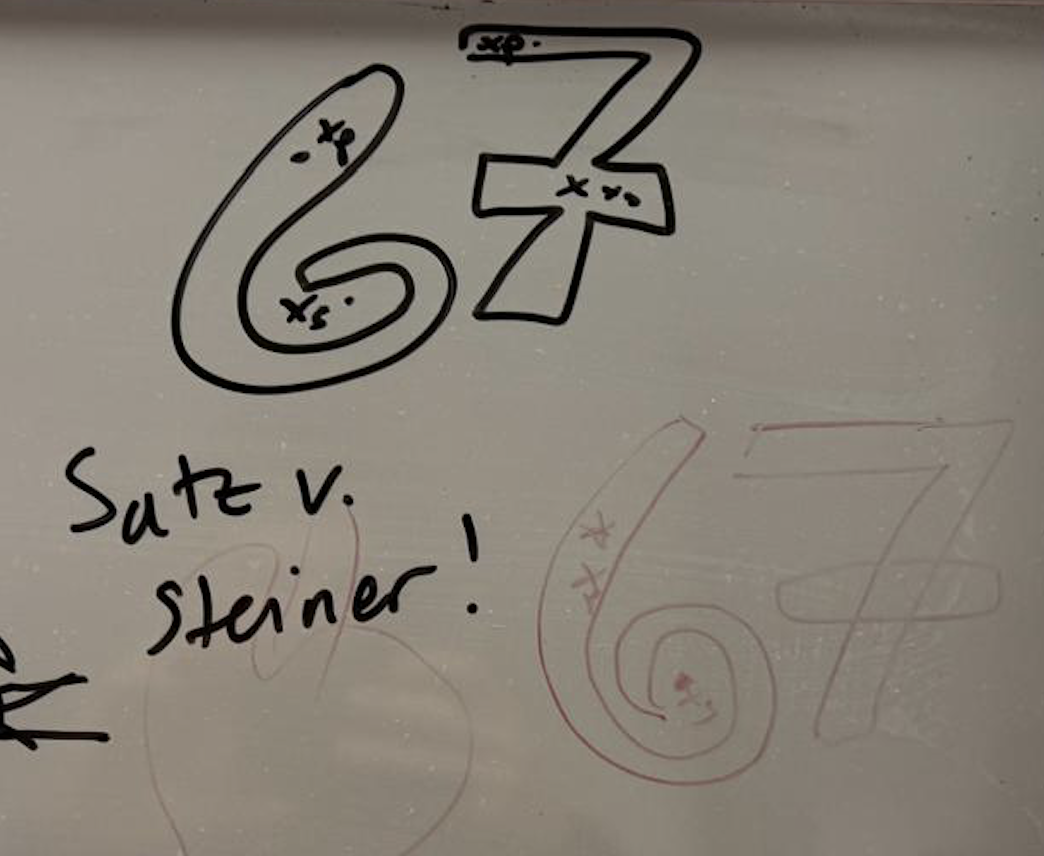
\includegraphics[width=0.5\textwidth]{img/steiner.png}
    \caption{Veranschaulichung des Steinerschen Satzes}
    \label{fig:steinerscher_satz}
\end{figure}

    
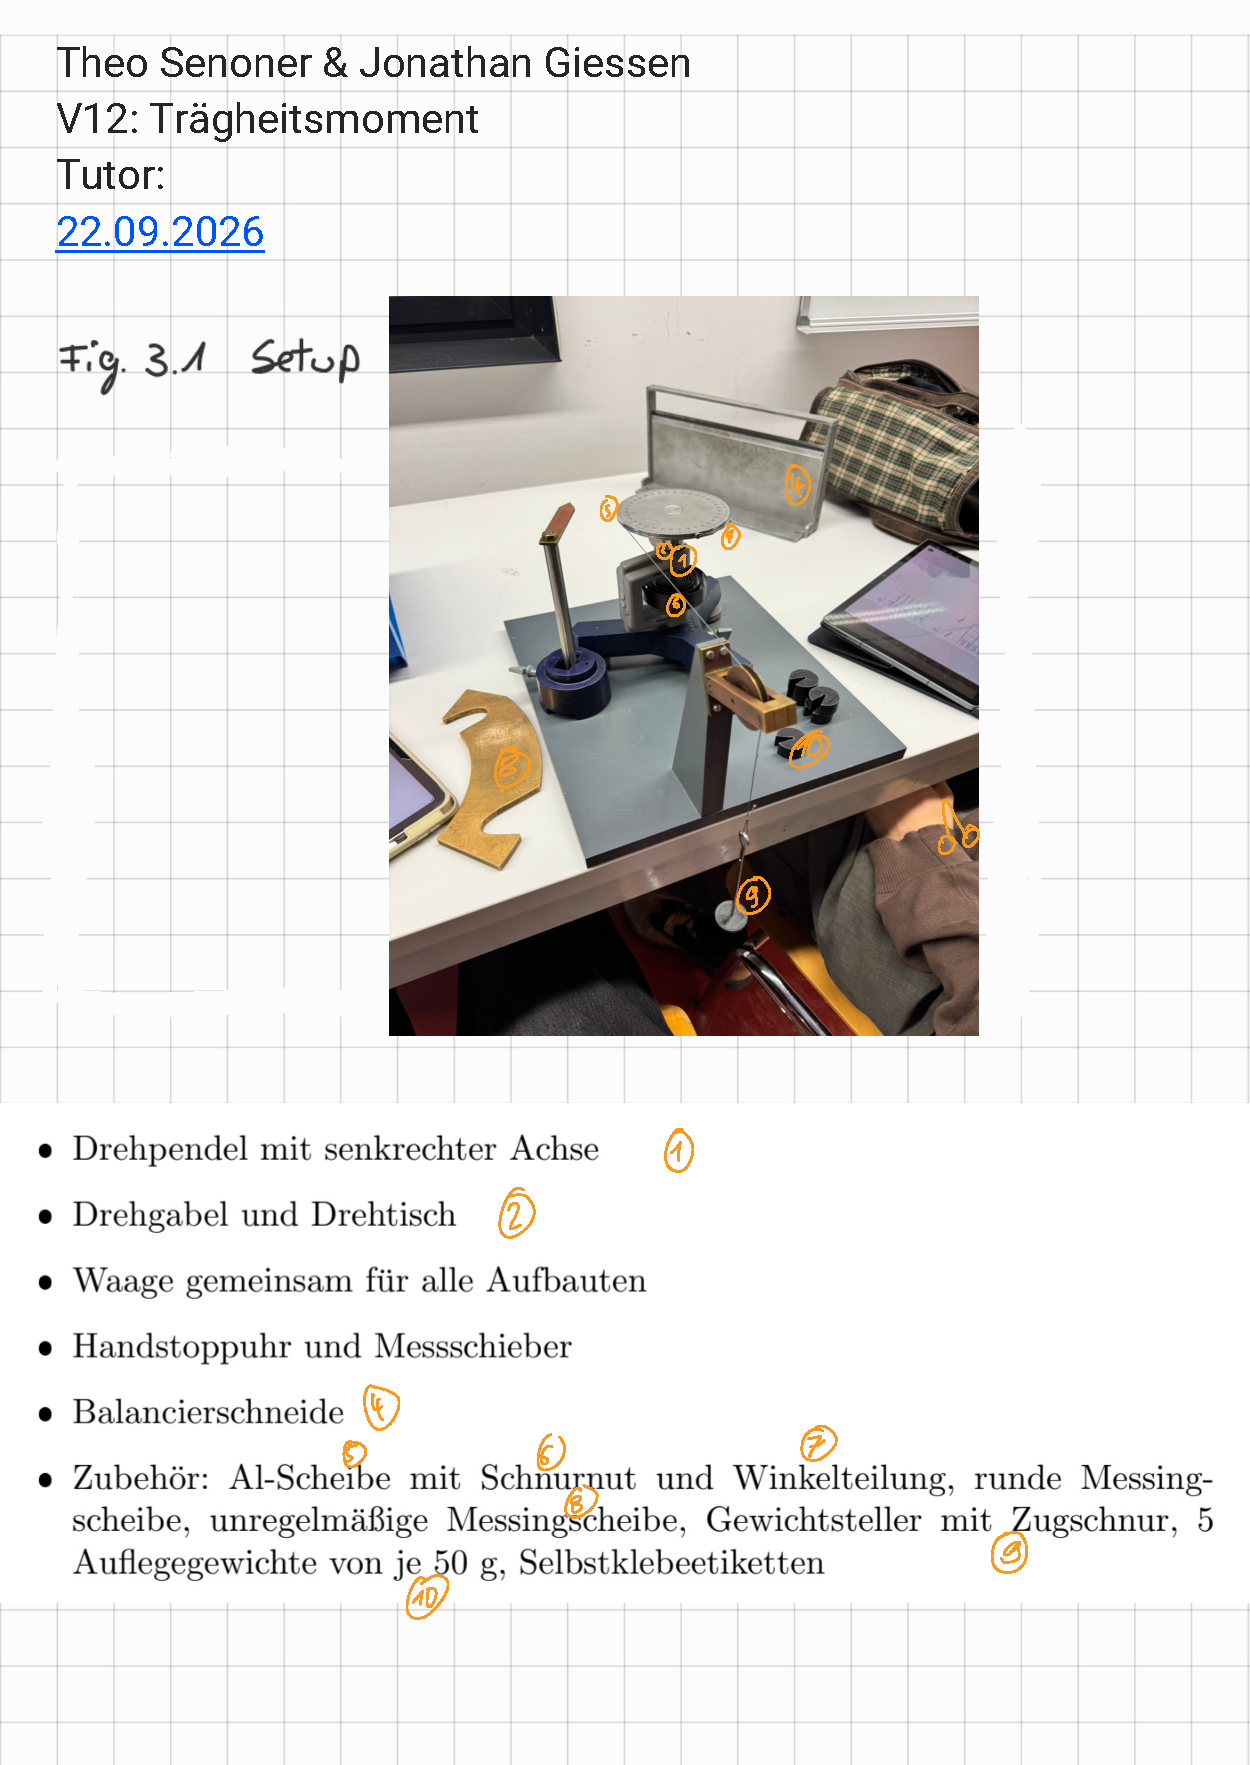
\includepdf[
    pages=-,
    width=\textwidth,
    height=0.95\textheight,
    keepaspectratio,
    pagecommand={\thispagestyle{scrheadings}},
    pagecommand*={\thispagestyle{scrheadings}\section{Messprotokoll}\subsection{Versuchsaufbau und Aufgaben}}
]{../Messprotokoll 12.pdf}

\pdftabelle{Messwerte für die statische Bestimmung des Richtmoments}{tab:richtmoment_messwerte}


\subsection{Durchführung}
Die praktische Durchführung gliedert sich in drei wesentliche Teile: die Bestimmung des Richtmoments, die Untersuchung des Schwerpunkts und Trägheitsmoments einer unregelmäßigen Platte sowie die Überprüfung des Steinerschen Satzes.

\paragraph{Bestimmung des Richtmoments (statisch und dynamisch)} 
Zur statischen Bestimmung des Richtmoments wurde eine Aluminiumscheibe mit Winkelskala auf der Drehachse fixiert. Über eine Schnur, die um die Scheibe gewickelt und über eine Umlenkrolle geführt wurde, griff tangential eine Kraft an. Durch schrittweises Auflegen von fünf $\qty{50}{\gram}$-Massen auf einen Gewichtsteller wurde das angreifende Drehmoment variiert und jeweils der resultierende Drehwinkel abgelesen. Der Radius der Scheibe wurde mit einem Messschieber bestimmt. \\
Für die dynamische Bestimmung wurde das Pendel mit einem Drehtisch versehen. Zunächst wurde die Schwingungsdauer $T_1$ des leeren Tisches durch dreimaliges Stoppen von je 20 Schwingungen ermittelt. Anschließend wurde eine runde Messingscheibe, deren Masse und Durchmesser vorab gemessen wurden, zentriert aufgesetzt und analog die Schwingungsdauer $T_2$ des Gesamtsystems bestimmt.

\paragraph{Schwerpunkt und Trägheitsmoment der unregelmäßigen Platte}
Um den Schwerpunkt der unregelmäßig geformten Messingplatte zu finden, wurde diese auf eine Balancierschneide gelegt. Durch das Ausbalancieren in zwei zueinander senkrechten Lagen konnten zwei Schwerelinien auf einem Klebeetikett markiert werden; ihr Schnittpunkt markierte den Schwerpunkt. Die Platte wurde mit diesem Schwerpunkt exakt über der Achse auf dem Drehtisch fixiert und ihre Schwingungsdauer gemessen, um das Trägheitsmoment $J_s$ zu ermitteln.

\paragraph{Messung zum Steinerschen Satz}
Zur Überprüfung des Steinerschen Satzes wurde auf dem Klebeetikett eine Gerade durch den zuvor bestimmten Schwerpunkt gezogen. Auf dieser Linie wurden fünf Punkte in unterschiedlichen Abständen $a_1$ bis $a_5$ zum Schwerpunkt markiert. Die Platte wurde nacheinander an diesen Punkten auf die Drehachse gesetzt. Für jeden Abstand wurde die Schwingungsdauer gestoppt, um die Zunahme des Trägheitsmoments durch die exzentrische Aufhängung zu dokumentieren. Abschließend wurde die Gesamtmasse der unregelmäßigen Platte mit einer Waage ermittelt.

\section{Auswertung}

\subsection{Aufgabe 1: Ermitteln des Richtmoments}
Die Messwerte für die statische Bestimmung des Richtmoments sind in Tabelle \ref{tab:richtmoment_messwerte} aufgeführt. 

Mithilfe der Funktion:
\begin{equation}
    y = m \cdot x + b
\end{equation}

wird ein linearer Zusammenhang zwischen dem Drehmoment $M$ und dem Drehwinkel $\phi$ angenommen. Die Steigung $m$ der Ausgleichgerade entspricht dem Richtmoment $D$.

\begin{figure}[H]
    \centering
    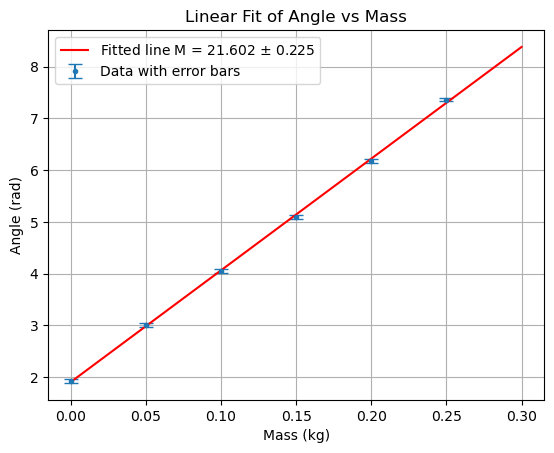
\includegraphics[width=0.8\textwidth]{img/A1.png}
    \caption{Ausgleichsgerade zur Bestimmung des Richtmoments}
    \label{fig:ausgleichsgerade_richtmoment}
\end{figure}

Die Steigung der Gerade beträgt $m = \qty{2.160(23)e-2}{\newton\meter\per\radian}$, was dem Richtmoment $D$ entspricht.



\clearpage

\listoffigures


\listoftables

\begin{thebibliography}{5}
    \bibitem{PAPskript} Dr. J.Wagner, \emph{Physikalisches Anfängerpraktikum}, Stand 11/2024
    \bibitem{ilberg1988physikalisches} W. Ilberg, M. Krötzsch, \emph{Physikalisches Praktikum für Anfänger}, BSB B. G. Teubner Verlagsgesellschaft, Leipzig (1985).
\end{thebibliography}




\begin{comment}

\begin{table}[H]
    \centering
    \caption{Mess- und Geräteparameter für die exemplarische Berechnung (Messung 28).}
    \label{tab:parameter_messung_28}
    \begin{tabular}{ll}
        \toprule
        \textbf{Größe} & \textbf{Wert} \\
        \midrule
        Fallstrecke & $s_1 = 10\,\text{Skt} = 5.00 \cdot 10^{-4}\,\text{m}$ \\
        Fallzeit & $t_1 = 11.85\,\text{s}$ \\
        Steigstrecke & $s_2 = 10\,\text{Skt} = 5.00 \cdot 10^{-4}\,\text{m}$ \\
        Steigzeit & $t_2 = 18.19\,\text{s}$ \\
        Skalenteilung & $1\,\text{Skt} = 5.00 \cdot 10^{-5}\,\text{m}$ \\
        Kondensatorspannung & $U = 500\,\text{V}$ \\
        Plattenabstand & $d = 6.00 \cdot 10^{-3}\,\text{m}$ \\
        Luftdruck & $p = 100285\,\text{Pa}$ \\
        Erdbeschleunigung & $g = 9.81\,\frac{\text{m}}{\text{s}^2}$ \\
        Dichtedifferenz & $\rho = \rho_{\text{Öl}} - \rho_{\text{Luft}} = 871.21\,\frac{\text{kg}}{\text{m}^3}$ \\
        Unkorrigierte Luftviskosität & $\eta_0 = 1.81 \cdot 10^{-5}\,\text{Pa}\cdot\text{s}$ \\
        Cunningham-Konstante & $b = 7.78 \cdot 10^{-3}\,\text{Pa}\cdot\text{m}$ \\
        \bottomrule
    \end{tabular}
\end{table}
\end{comment}
\end{document}